% Add something brief on news comment gap, add to title?
\section{Introduction}
\label{sec:introduction}

An online news article may attract hundreds of comments, but their ordering gives some contributions greater prominence than others. Which contributions appear depends on more than what readers write. Ordering by votes, posting time, `recommended', pinning Editors' Picks, and displaying or hiding replies all determine which perspectives receive prominence. The same discussion organised in different ways can therefore present different accounts of readers' responses to a story.

These choices extend editorial influence beyond the article itself. They involve algorithmic gatekeeping through the allocation of comment visibility and agenda-setting through the organisation of issue and attribute salience. Editors can manually highlight individual contributions, while ranking algorithms are responsible for distributing visibility across the remaining discussion. Reader votes supply another selection signal, but their influence depends on how the interface uses them. Prior work examines the characteristics of selected comments and the consequences of comment curation \citep{Diakopoulos2015,JuarezMiro2022,He2024,Wang2021}, but less is known about how ordering, pinning, and reply handling jointly shape the attributes and topics presented from the same comment pool. We examine these choices together, asking both what kinds of contributions they bring forward and whose topical priorities the resulting presentation resembles.

We focus our attention on two research questions:
\begin{enumerate}[label=RQ\arabic*]
\item How can algorithmic ordering, reply handling, and comment pinning change the attributes surfaced by a discussion, and how do these effects depend on the depth of the visible comments?
\item How can algorithmic ranking shift the visible topic distribution towards or away from journalist vs audience-derived agendas?
\end{enumerate}

To address these, we gather 2.39 million comments across 5,118 articles from 2025 from Austrian newspaper \textit{Der Standard}, one of the largest German-speaking news forums. We compare ranking algorithms across 90 combinations of ordering, reply presentation, and comment pinning. For RQ1, we develop the ``\textbf{F}eature-\textbf{O}riented \textbf{R}anking \textbf{U}tility \textbf{M}etric'' (FORUM) to measure which comment attributes are visible earlier under different ranking algorithms, relative to random, best-possible, and worst-possible feature orderings. With RQ2, we fit an article--comment topic model with BERTopic, and assess how different ranking algorithms represent the topics present in the discussion relative to the article and expressed reader preferences.

\section{Related Work}

\subsection{Algorithmic gatekeeping and agenda-setting}

Gatekeeping concerns the selection and access decisions through which some contributions reach public communication while others receive little or no visibility. Early work conceptualised this as journalists' selection of news events \citep{White1950}; later accounts describe the broader process through which information passes, or is closed off from, media attention \citep{ShoemakerVos2009}. In digital settings, journalists, users, and algorithms all participate in selection through platforms with different mechanisms \citep{Wallace2018}. Audience engagement can itself act as a gatekeeping signal, while ``gatewatching'' describes the collaborative monitoring and highlighting of already available information \citep{ShoemakerVos2009,Bruns2003}. On the Internet, gatekeeping power now extends to popular search engines and social networks \citep{Nielsen2016}. Audits of news curation likewise reveal systematic differences in the source diversity and topic composition produced by algorithmic and editorial selection \citep{BandyDiakopoulos2020}.

Agenda-setting theory, first developed by \citet{McCombs1972}, posits that mass media influence public opinion not by dictating what to think, but by making certain issues more salient than others in shaping what people think about. Building on this, second-level agenda-setting theory shifts the focus from issue salience to attribute salience---how media coverage influences the public's understanding of how to think about an issue, including its tone, framing, and associations \citep{McCombs1997}. Beyond first- and second-level effects, extensions examine networks of associated issues, influence between media, and how audiences shape and combine agendas in their information environments \citep{Guo2011,Atwater1987,Kim2006,Shaw1999}.

In the digital age, algorithmic systems have transformed news production and consumption, prompting a reconceptualisation of classic media theories and empirical studies \citep{VanDijck2013, Voinea2025}. Platforms now act as “algorithmic gatekeepers”---selecting, ranking, and personalising news and opinion pieces \citep{Wallace2018}. Increased attention is now being paid to their agenda-setting consequences. For instance, \citet{Trielli2022} show that Google search results during the 2020 U.S. election exhibited differences in topic salience compared to the news media agenda, with limited user power to reshape these. In a controlled experiment, \citet{Einarsson2025} find that personalised news recommendations subtly narrow the range of topics towards softer news in terms of both user exposure and consumption. Such studies demonstrate how ranking systems across platforms help shape what is emphasised in public discourse. We extend this perspective to comment sections: by analysing how ranking policies prioritise certain types of comments, we examine a form of algorithmic gatekeeping and agenda-setting in public discourse.

\subsection{Ranking and the governance of discussion}

Users often lack the time to scan hundreds of comments in online discussions, missing potentially interesting contributions and sometimes ending their participation altogether \citep{Levy2008, Lampe2014}. On some platforms, users view only 3\% of comments \citep{Althuniya2020}.
Beyond news comments, \citet{Piccardi2025} show in a field experiment on X that re-ranking posts changes exposure and affective polarisation, while audits comparing algorithmic and chronological feeds find differences in account visibility \citep{Efstratiou2026}. Feed audits also associate rank with substantial differences in subsequent activity \citep{Chan2026}. Such findings motivate examining ranking interventions, while our analysis concerns presentation rather than downstream attitudes.
Within comment sections, an exploratory audit has also found user-to-user variation in visible comment rankings, motivating more systematic study of how ranking shapes discourse \citep{Nutakki2026}.
Automated assessment and ranking are increasingly important \citep{Momeni2016}. For example, the German language focused AQuA \citep{Behrendt2024} combines predictions for 20 dimensions into a weighted deliberative quality score informed by expert and non-expert judgements. Ideally, users see a summary of the discussion through selected comments, though this is challenging without biasing the results. Many news organisations rank comments in reverse-chronological order by default, or allow sorting by user up/downvotes. Some run an \emph{Editors' Picks} section, where selected comments are made prominently visible to readers. 

Defaults matter because most users do not change comment sorting. Comment sorting can foster participation and constructive discussion \citep{Diakopoulos2011}, while highlighting high-quality contributions may improve commenters’ subsequent contributions \citep{Wang2021}. Negative evaluations can increase posting while lowering later quality \citep{Cheng2014}, and community responses to incivility depend on conditions supporting collective corrective action \citep{Ziegele2020}. Concentrated participation may also produce a more hostile visible tone \citep{KimNoh2026}.

Comment ranking and feedback influence which comments users read as well as write. Editor-picked comments provide a debate overview but may reflect undisclosed editorial policies. Community-based ranking can sanction incivility but may discourage minority opinions. This creates tension between audience participation and journalistic gatekeeping \citep{Chen2017, Diakopoulos2015}. Users' and editors' judgements often differ. \citet{JuarezMiro2022} discusses the ``comment gap''---only 17.2\% of New York Times comments made both the readers' and Editors' Picks lists, as readers favour direct, confrontational, and aligned comments, while editors chose more articulate, conciliatory, and diverse ones. Using approximately 80,000 New York Times articles, \citet{He2024} find that Editors' Picks tend to be longer, more article-relevant, more positive, and less toxic than other comments, with selection criteria varying across news sections. Whilst the majority of this closely related work is in English, efforts to expand analysis through data work have also emerged in German, such as \citet{Fraxanet2026}'s \textit{Der Standard} 2013--2022 forum archive. Together, these studies motivate examining further how different algorithmic factors jointly shape the attributes and topics made prominent within a fixed discussion.

\section{Data and Methods}
\label{sec:data}
\subsection{Data collection}
\textit{Der Standard} is one of Austria's two most-read ``quality-newspapers'' (``qualitätszeitung'', roughly equivalent to a ``broadsheet''), hosting one of the largest German-speaking online forums globally with 73,000 active users annually \citep{Burger2022}. Our analysis uses the publicly accessible articles and comments from stories in the year 2025. Reading is publicly available, while commenting and voting require registration (pseudonymously, if desired). Pinned posts (or ``Editors' Picks'') in discussions are comments deemed especially valuable by editors, community management, or community guides\footnote{``Editors'' here includes the journalist(s) who wrote the article. ``Community management'' are \textit{Der Standard} employees in charge of a small number of volunteer ``Community guides'' who also assist with content moderation \citep{DerStandard2021}}. They are shown at the top of the discussion and marked as \emph{pinned} (``\emph{Angeheftet}'').

Our data collection uses the same underlying corpus and collection pipeline as the companion study \citep{CommentGap1}. We programmatically collected accessible articles published in 2025 and their public comment records using monthly sitemaps and the site's public GraphQL endpoint, retaining comment text, hashed author usernames, comment relationships, posting timestamps, vote totals, and pinned status, alongside article text and metadata. The initial collection contains 9,415,942 comment records, including 193,090 deleted-comment tombstones. We also collected December 2024 records for author-history features, excluding them from the 2025 outcome sample. We focus our analysis on discussions containing at least one comment selected as Editors' Pick and at least one non-selected comment. From 44,596 retrieved articles, the final sample contains 5,118 discussions with 2,392,952 candidate comments, of which 20,930 are Editors' Picks. The mean number of comments per discussion is 467.6 (median 325), and the mean number of Editors' Picks is 4.09 (median four). Combining up- and downvotes, the mean total is 7.06 votes per candidate comment (median two). We use one common article split for all selector models: 2,559 development and 2,559 held-out articles, stratified by publication month and joint candidate-size tercile. The policy and topic analyses, as the focus of this paper, use the held-out partition and additionally require more than 10 comments in a discussion, leaving 2,556 discussions and 1,203,611 comments.

\subsection{Constructing ranking algorithms}
\label{sec:policies}
We define different possible comment ranking policies. Each comment ranking algorithm is made up of three policy elements: primary ordering, Editors' Pick status, and reply structure. Primary ordering is the main way in which comments are ranked relative to each other (e.g. in order of upvotes, time posted, etc.). Replies may be displayed ``loose'' (unattached to their parents), in tree form (attached to their parents), or hidden (only root comments are shown). Editors' Picks may be pinned to the top of the discussion or unpinned, and replies to pinned comments are hidden for presentation purposes. By default \textit{Der Standard} displays comments in reverse-chronological order, with Editors' Picks pinned and replies displayed in tree form.

We evaluate fourteen substantive primary orderings: relative votes (upvotes - downvotes), upvotes, chronological, reverse chronological, and ten predictive orderings. Predictive comment-ranking models are carried forward from \citep{CommentGap1}: conditional logit, XGBoost with and without BGE-M3 text features, and neural ranking models with and without BGE-M3 text features. Each model variant supplies audience- and editor-score orderings: the editorial labels are observed Editors' Picks, while the audience labels select an equally sized top-$k$ set by relative votes. The models share 41 scalar textual, contextual, author-history, reply-structure, and deliberative predictors (21 non-AQuA inputs plus 20 raw expected AQuA dimension scores; Appendix~\ref{app:development}). Text-enabled variants additionally use fixed BGE-M3 comment embeddings \citep{chen2024m3}. Conditional logit uses article--selector strata; boosted trees and neural networks learn ranking scores. We use the predicted comment scores from the models for ordering, without refitting to the held-out data. An explicit random ordering supplies a fifteenth condition. Crossing these with three reply modes and two pinning states gives $15\times3\times2=90$ final algorithms: 84 substantive algorithms and six random controls.

For FORUM, substantive ordering scores can tie for several comments, so we calculate ten seeded deterministic tie-breaking draws and average them. The random controls have no score ties; we instead generate 100 seeded permutations. These repeated presentations average over arbitrary ordering choices, while the separate 2,000 discussion-bootstrap draws quantify uncertainty across discussions.

\subsubsection{Outcome features}
We evaluate ten primary comment-level outcomes (Table~\ref{tab:outcome-features}), each scored separately rather than collapsed into a single quality index. Together they span deliberative quality and safety, topical relevance and novelty, affect, language form and readability, and participant history. This breadth exposes normative trade-offs---for example, a policy may increase comment--article relevance while reducing novelty---without treating any one measurable attribute as the definition of a good comment.

\begin{table}[t]
\centering
\small
\begin{tabular}{@{}p{0.30\linewidth}p{0.65\linewidth}@{}}
\toprule
Outcome & Operationalisation \\
\midrule
AQuA deliberative quality & Weighted composite of 20 expected ordinal AQuA dimension scores (each scored 0--3), on a 0--5 scale \citep{Behrendt2024}. \\
Comment--article similarity & Mean of the three largest cosine similarities between the comment's BGE-M3 embedding and embeddings of article passages (nonempty title, subtitle, or body-paragraph segments). \\
Toxicity & Maximum predicted toxicity probability across comment chunks from the TextDetox XLM-R Large Toxicity Classifier v2 \citep{textdetox2024xlmr}. \\
Author incumbency & $\log(1+n_{30})$, where $n_{30}$ is the author's number of comments on other articles in the preceding 30 days. \\
Prior audience reception & $R_{30} = \log\!\left((U_{30}+0.5)/(D_{30}+0.5)\right)$, where $U_{30}$ and $D_{30}$ are the number of up/downvotes on the author's comments on other articles in the preceding 30 days. \\
Comment novelty & Mean cosine distance to the five nearest other comments in the completed discussion, excluding the comment itself. \\
Positive and negative sentiment & Separate positive and negative probabilities from CardiffNLP XLM-R; long comments use a token-weighted mean over chunks \citep{cardiffnlp2022xlmr}. \\
Lexical diversity & Corrected type--token ratio, $\mathrm{CTTR}=V/\sqrt{2N}$, where $V$ is the number of distinct word types and $N$ the number of word tokens \citep{Benoit2018}. \\
Reading difficulty & Raw SMOG-DE, $\sqrt{30P/S}-2$, where $P$ is the number of polysyllabic words and $S$ the number of sentences, with German syllabification \citep{Benoit2018,bamberger1984lesen}. \\
\bottomrule
\end{tabular}
\caption{Ten primary comment-level outcomes. The sentiment row contains two separately analysed outcomes.}
\label{tab:outcome-features}
\end{table}

\subsection{Measuring feature gatekeeping}
\subsubsection{FORUM}
The subsequent analysis of different ranking algorithms is partly inspired by \citet{Young2021}, who compared sorting policies on a debating website with regard to winning arguments in argumentation theory. For each discussion, we order the comments according to each ranking policy. We use the ``\textbf{F}eature-\textbf{O}riented \textbf{R}anking \textbf{U}tility \textbf{M}etric'' (FORUM) that measures how well a ranking policy $p$ surfaces the highest-scoring comments in a discussion according to a feature $f$. The metric compares how the ordering of comments $o^p$ under policy $p$ compares to the best-possible ordering ($o^b$ - descending order of score $f$), worst-possible ordering ($o^w$ - ascending order of score $f$), and the expected random baseline. Here we describe how FORUM is calculated for a ranking policy $p$ with feature $f$ on a particular discussion on a news article.

Let $t_i^p$ denote the cumulative feature value of $f$ through to comment at rank $i$ under policy $p$, and let $T$ be the total over $N$ candidates. The expected random trajectory is $t_i^r=iT/N$. Descending and ascending feature orders give the attainable upper and lower trajectories $t_i^b$ and $t_i^w$. The normalised cumulative score at rank $i$ is
\begin{equation}
\gamma_i^p=\begin{cases}
(t_i^p-t_i^r)/(t_i^b-t_i^r),&t_i^p>t_i^r,\\
(t_i^p-t_i^r)/(t_i^r-t_i^w),&t_i^p<t_i^r,\\
0,&t_i^p=t_i^r.
\end{cases}
\end{equation}
This is visualised in Figure~\ref{fig:forum}. If a policy tends to return higher scored comments earlier than expected at random, the line tracking cumulative score will fall above the diagonal baseline. If the policy tends to return higher scoring comments later than expected at random, then it will fall below the baseline. The normalised deviation $\gamma_i^p$ compares the cumulative feature value through rank $i$ with the best-, worst-, and random-order trajectories. It therefore measures the cumulative prominence of the first $i$ comments, rather than how the $i$ comments themselves are ordered. We measure how a policy $p$ ranks up to depth $d$ by taking the \emph{average} $\gamma_i^p$ over all ranks through $d$. Thus, FORUM at depth $d$ is:
\begin{equation}
F_d^p=\frac{1}{d}\sum_{i=1}^{d}\gamma_i^p.
\end{equation}
In our analysis, we measure FORUM at two depths: the first ten comments and the full discussion. FORUM lies in $[-1,1]$: values near $1$ indicate an ordering close to the best attainable feature trajectory, values near $-1$ one close to the worst, and values near zero no systematic departure from random. Because it uses feature values and separate best- and worst-side normalisation, it is not simply a rank-correlation measure. Whether a positive score is desirable depends on the outcome (e.g. with toxicity). Because the random, best, and worst trajectories coincide at $N$, the final rank is degenerate; we therefore define the full-discussion score as the average through the last nontrivial rank, $F_{N-1}^p$.

In cases where a ranking policy removes comments from immediate view, such as the ``hide replies'' functionality, we choose to interpolate a straight line from the cumulative feature score of the final visible comment up to the total cumulative feature score $T$ in the process of calculating $F_d$. This allows comparison between ranking policies over a different number and set of comments. Practically, this is akin to a situation where any one of the hidden comments is equally likely to be viewed next by a reader (if they choose to click any to expand). Positive and negative deviations have different attainable denominators, so realised random permutations need not average to exactly zero. We therefore retain empirical random controls when interpreting policy contrasts.
\begin{figure}[t]
\centering
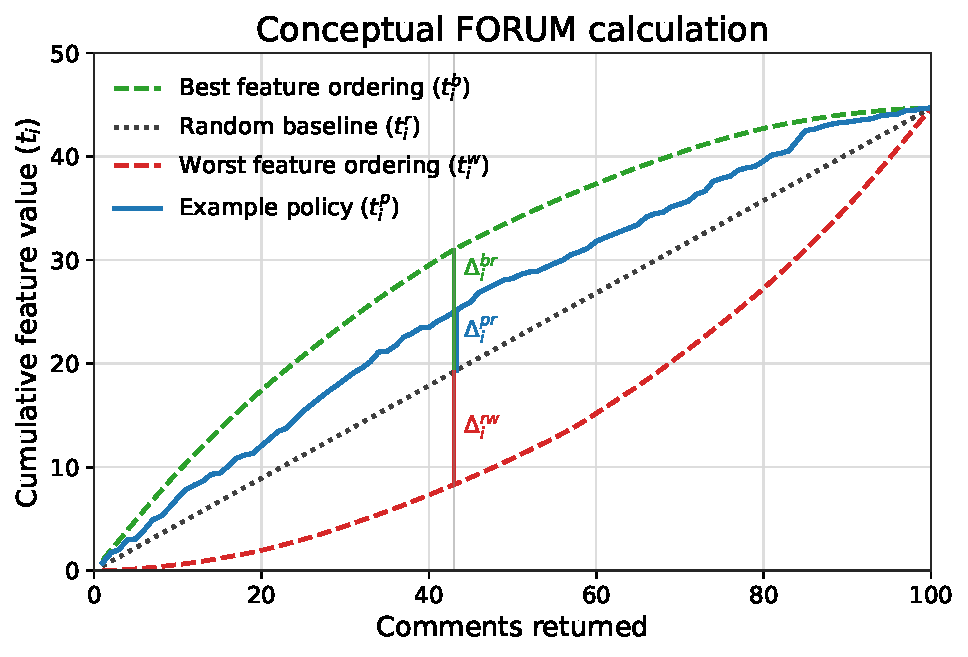
\includegraphics[width=\linewidth]{figures/feature_score.pdf}
\caption{Conceptual FORUM calculation. $\Delta^{xy}_i = t^x_i - t^y_i$. The cumulative feature value under an example policy is compared with the random baseline and the attainable best and worst feature orderings; the normalised deviation at rank $i$ is then averaged through depth $d$.}
\label{fig:forum}
\end{figure}

The top-10 / full discussion FORUM scores use discussion-averaged scores for each ranking policy and outcome feature. To understand the systematic effect of each factor in a ranking algorithm, we use paired contrasts to estimate the average effect of each. Ordering contrasts compare each ordering with random while averaging over the six reply/pinning variants. Reply contrasts compare trees or hidden replies with loose presentation, averaging over ordering and pinning. Pinning contrasts average over ordering and reply mode. We retain detailed effects for all policy combinations in Appendix~\ref{app:ordering}. We use 2,000 seeded discussion-bootstrap draws for percentile intervals. 

\subsubsection{Clustering policies by presented feature profiles}

To gain a greater understanding of how different ranking algorithms are similar / dissimilar from each other, we perform a clustering analysis of them based on the FORUM scores for all 41 of the common scalar features for the predictive models (as opposed to the 10 outcome features previously studied). Each of the 90 algorithms is represented by its discussion-averaged FORUM scores on each of the 41 feature axes (separate clusterings performed for top-10 and full discussion). At each depth, a ten-dimensional UMAP embedding \citep{McInnes2018UMAP} with 15 neighbours and minimum distance zero is clustered with HDBSCAN \citep{Campello2013HDBSCAN}, using minimum cluster size six, minimum samples three, and excess-of-mass cluster selection. We visualise the resulting clusters in two-dimensional UMAP embeddings (15 neighbours, minimum distance 0.15).

\subsection{Measuring the presented topic agenda}
\label{sec:topics}
\subsubsection{Article--comment topic model}
We fit BERTopic \citep{Grootendorst2022BERTopic} to BGE-M3 embeddings \citep{chen2024m3} of 48,887 article passages (a nonempty article title, subtitle, or body-paragraph segment) and an equally sized sample of 48,887 published comments from the held-out corpus. Comments are sampled round-robin across discussions in hashed order: we take the first hashed comment from each discussion, then the second, and so on, with stable hash tie-breaking within each round. This limits the influence of large discussions and makes the sample reproducible from the same corpus and hashing procedure. The mixed corpus gives article passages and sampled comments equal weight in topic discovery.

Appendix~\ref{app:topic-model} reports the coverage/stability comparison across different parameters used to assess the configuration. The selected configuration uses cosine-distance UMAP with ten neighbours and five components, followed by HDBSCAN with minimum cluster size 15, minimum samples five, and seed 2026. Automatic topic reduction yields 439 non-outlier topics; outliers remain unassigned. The final transformed corpus contains 48,887 article passages and 1,203,611 comments, of which 53.59\% and 26.64\%, respectively, receive valid topic assignments. The configuration balances stability, coverage, and topic granularity (Appendix~\ref{app:topic-model}). The low comment coverage can be largely explained through a large number of true outlier non-substantive comments, e.g., ``I agree'', ``What's your point?''. The agenda analysis includes 2,531 discussions with both an article and a complete-discussion topic distribution. This is a smaller sample than the feature analysis because both distributions require at least one topic assigned document. Topic-distribution mass for an article / discussion is renormalised to exclude topic outliers.

\subsubsection{Vote-activity weighting}
We estimate a proxy for attention at each rank from total votes (upvotes plus downvotes) at each visible rank under reconstructed reverse-chronological/tree/pinned presentation (default at \textit{Der Standard}). Within each development discussion, each visible rank receives its share of that discussion's visible vote total; we then average these shares equally across discussions and fit a smoothed empirical spline on 2,553 discussions. Hidden comments contribute neither ranks nor votes. The length-conditioned model is
\begin{equation}
p(r\mid L)=\frac{w_r}{\sum_{u=1}^{L}w_u},
\end{equation}
where $r$ is visible rank, $L$ is the number of comments visible under policy $p$, and $w_r$ is the frozen nonnegative rank weight. Log weights are represented by a cubic B-spline of log rank with a second-difference penalty. Nested development-fold validation selects smoothing; the final spline is refitted on all development discussions. For each policy, we renormalise the frozen weights over its visible length $L$, so they describe relative allocation among the comments exposed by that policy; omitted comments receive no visible rank or weight. Appendix~\ref{app:attention} gives the fit and its length-adjusted curves. These weights are a simple estimate of attention, not measured attention or a causal position effect. Votes combine age, content, prior prominence, and social feedback, among other factors which we are unable to capture or account for.

We compute article and complete-discussion topic distributions (unaffected by ranking). $A_j$ is the equally weighted mean of valid article-passage topic vectors for discussion $j$, and $C_j$ is the equally weighted mean of valid topic vectors over all eligible comments in that discussion; outliers are excluded and each distribution is renormalised. For a given ranking algorithm, we employ a weighted average of the topics of the visible comments, with weights reflecting expected attention at each rank. For discussion $j$, policy $p$, and presentation draw $b$, let $q_{jprb}$ be the topic vector of the comment at visible rank $r$, $w_r$ be the weight for that rank, and $a_{jprb}$ indicate a valid topic assignment. The visible topic distribution is
\begin{equation}
V_{jpb}=\frac{\sum_{r=1}^{L_{jpb}}w_r a_{jprb}q_{jprb}}
{\sum_{r=1}^{L_{jpb}}w_r a_{jprb}},
\end{equation}
where $L_{jpb}$ is the number of visible comments. Outlier comments may occupy ranks and consume weight but do not contribute topic mass. We retain ten pseudo-random permutations generated from fixed seeds, making substantive tie-breaking reproducible; random controls use 25 seeded permutations. Paired 95\% percentile intervals use 2,000 discussion-bootstrap draws. This visible topic distribution captures the visible weighted topic agenda under a ranking policy, as opposed to the full discussion unweighted topic distribution.

\subsubsection{Article versus relative-vote agenda similarity}
We measure how each policy changes similarity to two reference agendas: the article distribution $T_j^{\mathrm{article}}$ and a relative-vote distribution $T_j^{\mathrm{votes}}$, obtained by averaging the weighted visible distributions over ten relative-vote draws with loose replies and no pinning. Let $R$ denote random ordering with loose replies and no pinning. For either target $T_j$, the cosine gain is
\begin{equation}
g_{jp}(T_j)=\mathbb{E}_b\cos(T_j,V_{jpb})-
\mathbb{E}_b\cos(T_j,V_{jRb}).
\end{equation}
Positive gain indicates greater similarity to the target than under the common random baseline. Article alignment is measured by $g_{jp}(T_j^{\mathrm{article}})$; the difference $g_{jp}(T_j^{\mathrm{article}})-g_{jp}(T_j^{\mathrm{votes}})$ indicates whether a policy gains more towards the article or the vote-derived agenda.

For both outcomes, we report average paired effects across discussions. Ordering effects compare each ordering with random within the same reply/pinning configuration, then average over the six configurations. Reply effects compare trees or hidden replies with loose presentation; pinning effects compare pinned with unpinned presentation, averaging over substantive orderings and the remaining factor. The oracle is evaluated on both outcomes against $R$. Intervals use 2,000 discussion-bootstrap draws. The two-target scatter instead shows mean gains for each complete policy bundle; points below its diagonal have larger article-directed gains.

\subsubsection{Article agenda oracle}

A discussion's available comments may not permit an ordering that matches or even gets close to the article's topic distribution. We therefore construct an article-aware, best-found benchmark under the same rank-weighting scheme. The heuristic tries to maximise article--visible cosine similarity by ordering comments without any constraints. Greedy refinement starts from the article-affinity order, the 14 structured policy orders, and eight seeded random permutations, with up to five refinement iterations, four perturbation attempts per iteration, a 10\% perturbation fraction, and two local moves. Invalid-topic comments may occupy positions but contribute no topic mass. This result is a heuristic benchmark for comparison rather than a mathematical upper bound on attainable alignment.

\section{Results}

\begin{figure*}[h]
\centering
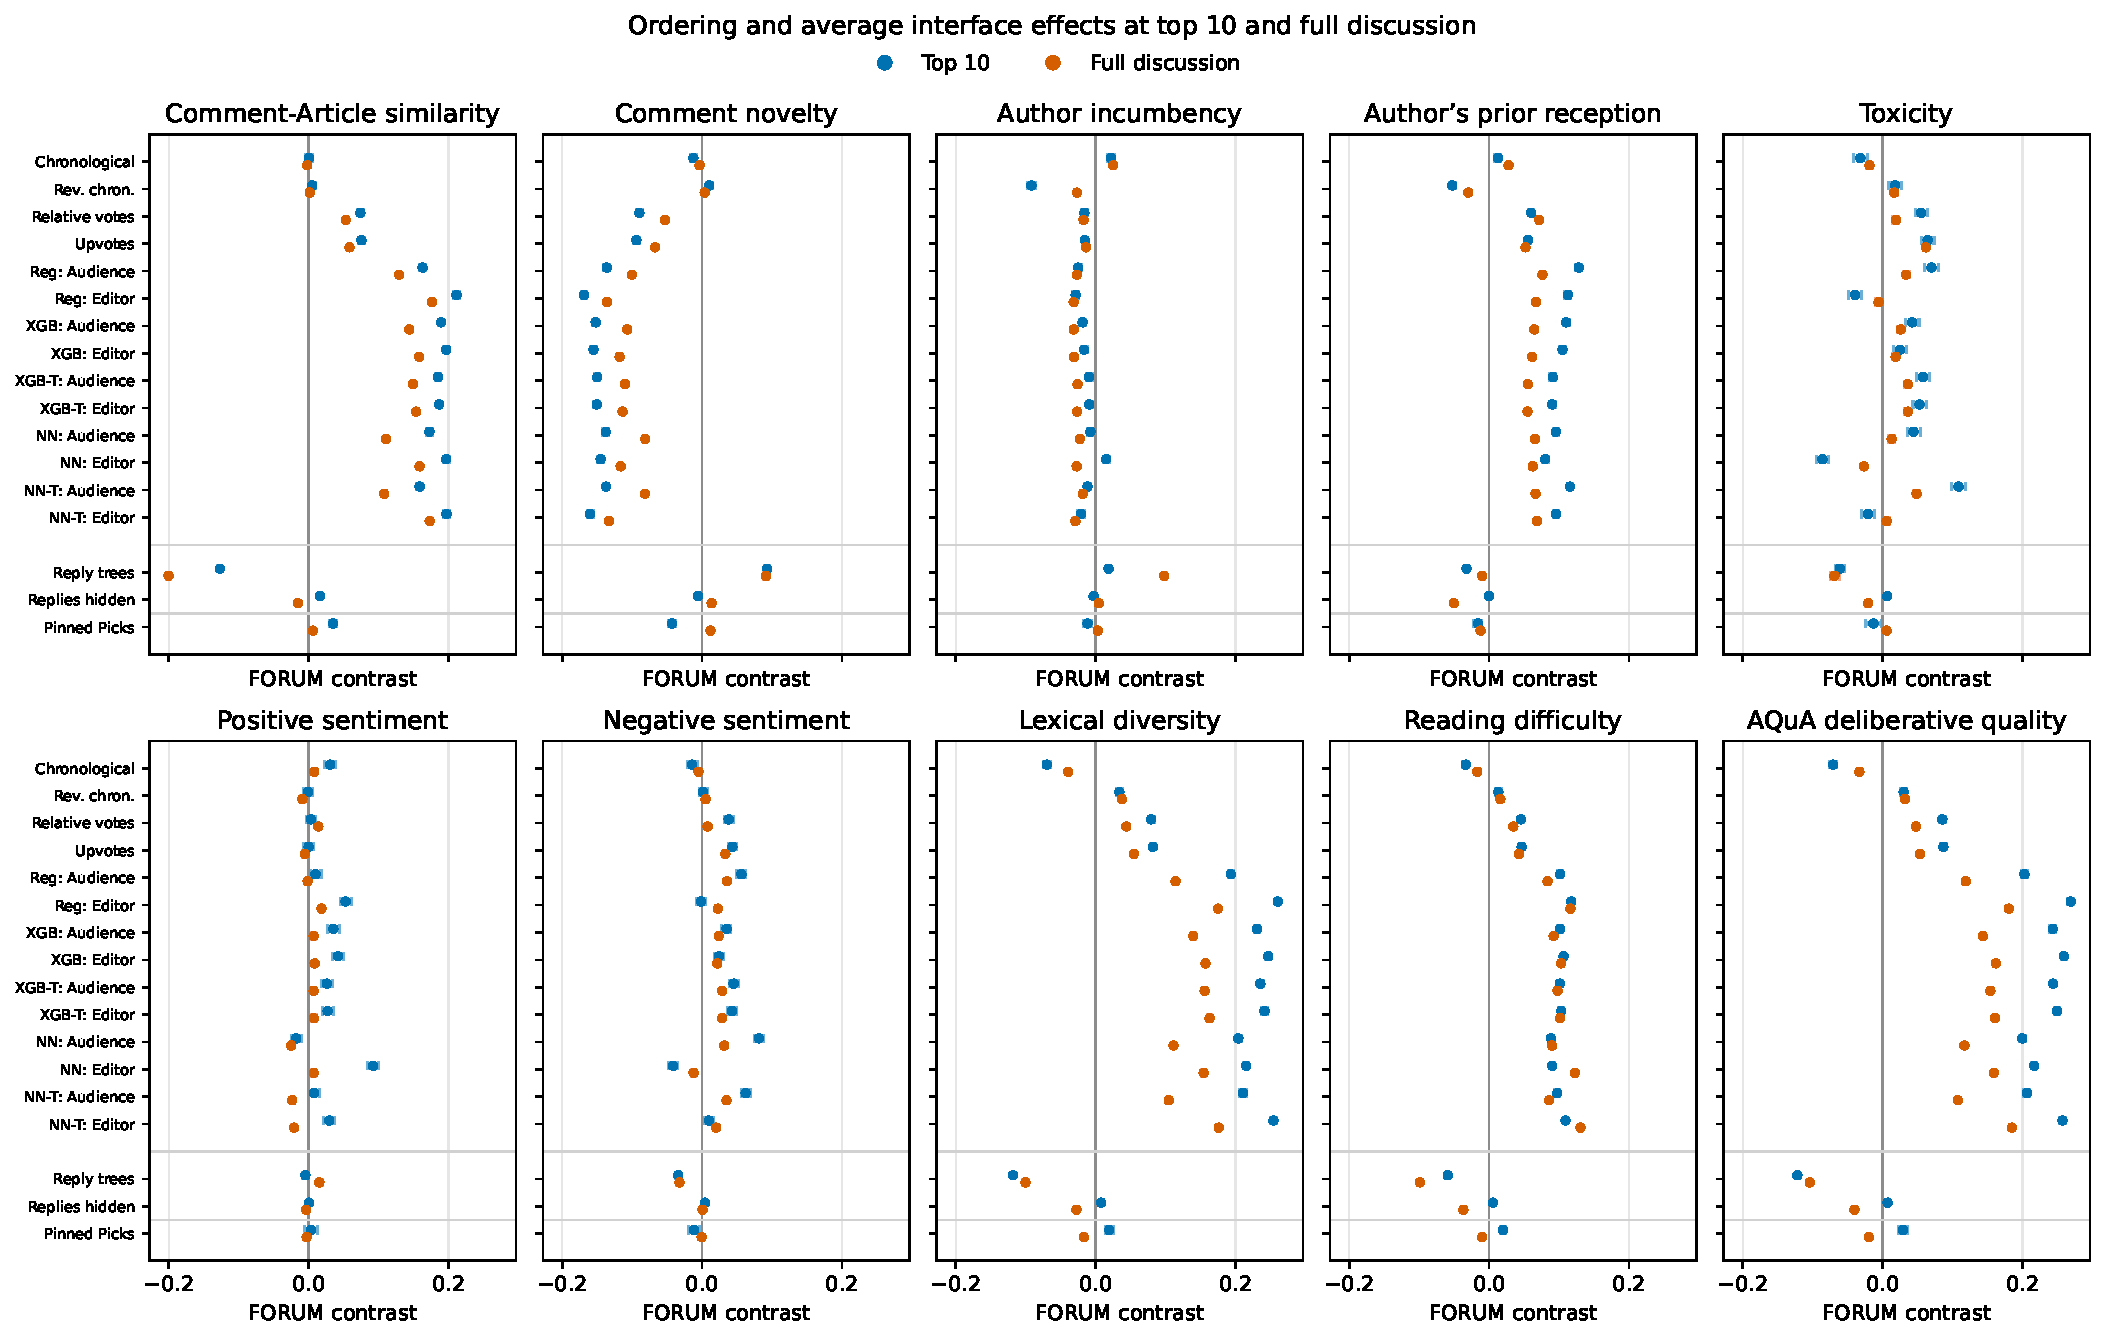
\includegraphics[width=\linewidth]{figures/ordering_and_interface_effects.pdf}
\caption{Ordering and average interface effects for ten primary attributes at both depths. Points compare orderings with random; interface contrasts average across the other policy factors. Points and intervals are paired 95\% discussion-bootstrap intervals.}
\label{fig:ordering-effects}
\end{figure*}

\subsection{Algorithmic gatekeeping}
The feature analysis addresses RQ1 by comparing ordering and interface effects at two depths.

\subsubsection{Ordering and interface effects on presented features}
We highlight AQuA, article similarity, and CTTR as they represent deliberative quality, article alignment, and textual form; semantic novelty illustrates a countervailing effect. Figure~\ref{fig:ordering-effects} shows average ordering and interface effects across all ten outcomes. At top 10, regression-editor ordering raises the FORUM score for AQuA by $0.2691$ (95\% CI $0.2652$--$0.2727$), article similarity by $0.2115$ ($0.2077$--$0.2154$), and CTTR by $0.2605$ ($0.2568$--$0.2643$). Relative-vote ordering produces smaller gains for the same outcomes: $0.0855$ ($0.0810$--$0.0897$), $0.0741$ ($0.0701$--$0.0780$), and $0.0794$ ($0.0755$--$0.0835$).

Interface effects are likewise feature-specific. Relative to loose presentation at top 10, intact reply trees reduce the FORUM score for AQuA by $0.1219$ (95\% CI $-0.1251$ to $-0.1187$), article similarity by $0.1268$ ($-0.1295$ to $-0.1239$), and CTTR by $0.1181$ ($-0.1207$ to $-0.1153$), while increasing semantic novelty by $0.0931$ ($0.0900$--$0.0958$). Over the full trajectory, the tree penalty for article similarity is larger ($-0.2002$, $-0.2036$ to $-0.1968$), whereas hiding replies reduces AQuA by $0.0402$ ($-0.0420$ to $-0.0384$) and pinning reduces AQuA by $0.0197$ ($-0.0216$ to $-0.0177$). Thus the same policy can look different at different exposure horizons. Positive FORUM means earlier prominence of larger values of the named feature; it does not mean that every larger value is desirable, as with toxicity.

Across the ten outcomes, predictive models consistently increase deliberative quality, article similarity, lexical diversity, reading difficulty, and prior audience reception at both depths, while reducing semantic novelty. Sentiment, toxicity, and author incumbency show weaker and more model- and horizon-dependent patterns. The three highlighted outcomes therefore illustrate the common positive movement, while novelty and the remaining outcomes show why it cannot be interpreted as a general improvement.

\subsubsection{The default presentation}
The default at \textit{Der Standard} combines reverse-chronological ordering, reply trees, and pinned Editors' Picks. Its top-10 FORUM scores indicate earlier prominence for AQuA ($0.303$), article similarity ($0.293$), and CTTR ($0.268$), alongside suppression of toxicity ($-0.385$) and semantic novelty ($-0.226$). These patterns weaken over the full discussion: the corresponding scores are $0.078$, $0.114$, $0.089$, $0.043$, and $-0.042$, with toxicity changing sign. Prior audience reception also changes sign, from $0.034$ to $-0.023$. 

\subsubsection{Policies with similar overall effects}
Clustering the 41-feature FORUM profiles yields four top-10 clusters, containing 32, 18, 22, and 18 distinct ranking algorithms, with no outliers (Fig.~\ref{fig:policy-clusters}). At full depth, the same procedure identifies seven clusters and four noise points. Across both depths, pin status (fill) and reply mode (shape) appear to act as strong separators in this space, with smaller scale groupings by ordering (colour). At top 10, one cluster contains all 15 unpinned tree bundles and another contains all 15 pinned tree bundles; the learned loose and hidden bundles are further separated largely by pinning, with 18 of the 20 unpinned learned loose/hidden bundles forming a distinct cluster. In the full depth clustering, one cluster contains all twenty loose-presentation algorithms based on predictive models. Hidden-reply bundles occupy distinct groups. The four outlier points are the loose relative-vote and upvote policies with and without pinning.

% FORUM thus supports comparison of policies by what they present, rather than grouping them only by the algorithm used to calculate scores. The depth-specific results also show why a single policy taxonomy is insufficient, as interface distinctions and similarities depend on how far through the discussion the evaluation extends.

\subsection{Algorithmic agenda-setting}
This analysis addresses RQ2 by comparing the alignment of the presented topic distributions.

\subsubsection{Topic agenda shifts}
Figure~\ref{fig:article-cosine-gain} shows average policy effects on article-directed cosine gain. Predictive models increase alignment relative to random ordering under matched reply/pinning configurations. The regression-editor ordering has an effect of $+0.0077$ (95\% CI 0.0063--0.0091), and the neural-editor ordering has an effect of $+0.0075$ (0.0061--0.0089). Relative votes and upvotes produce smaller point estimates, $+0.0019$ (0.0007--0.0030) and $+0.0016$ (0.0005--0.0028). Chronological and reverse-chronological ordering have intervals spanning zero. For scale, the mean random/loose/unpinned-to-oracle gap is $0.0860$; the conditional-logit and neural editor effects are about 8.9\% and 8.7\% of that benchmark gap.

Reply handling produces a larger shift. Hiding replies increases article-directed cosine gain by $+0.0286$ (0.0252--0.0318), whereas intact trees reduce it by $-0.0036$ ($-0.0043$ to $-0.0030$). Pinning increases it by $+0.0027$ (0.0011--0.0043). Relative to the same $0.0860$ benchmark gap, the hidden-reply and pinning effects are about 33.2\% and 3.1\%; intact trees move in the opposite direction. These ratios compare effect magnitudes with a common heuristic benchmark; they are not fractions of a known optimum attained by a particular policy bundle.

\begin{figure*}[h]
\centering
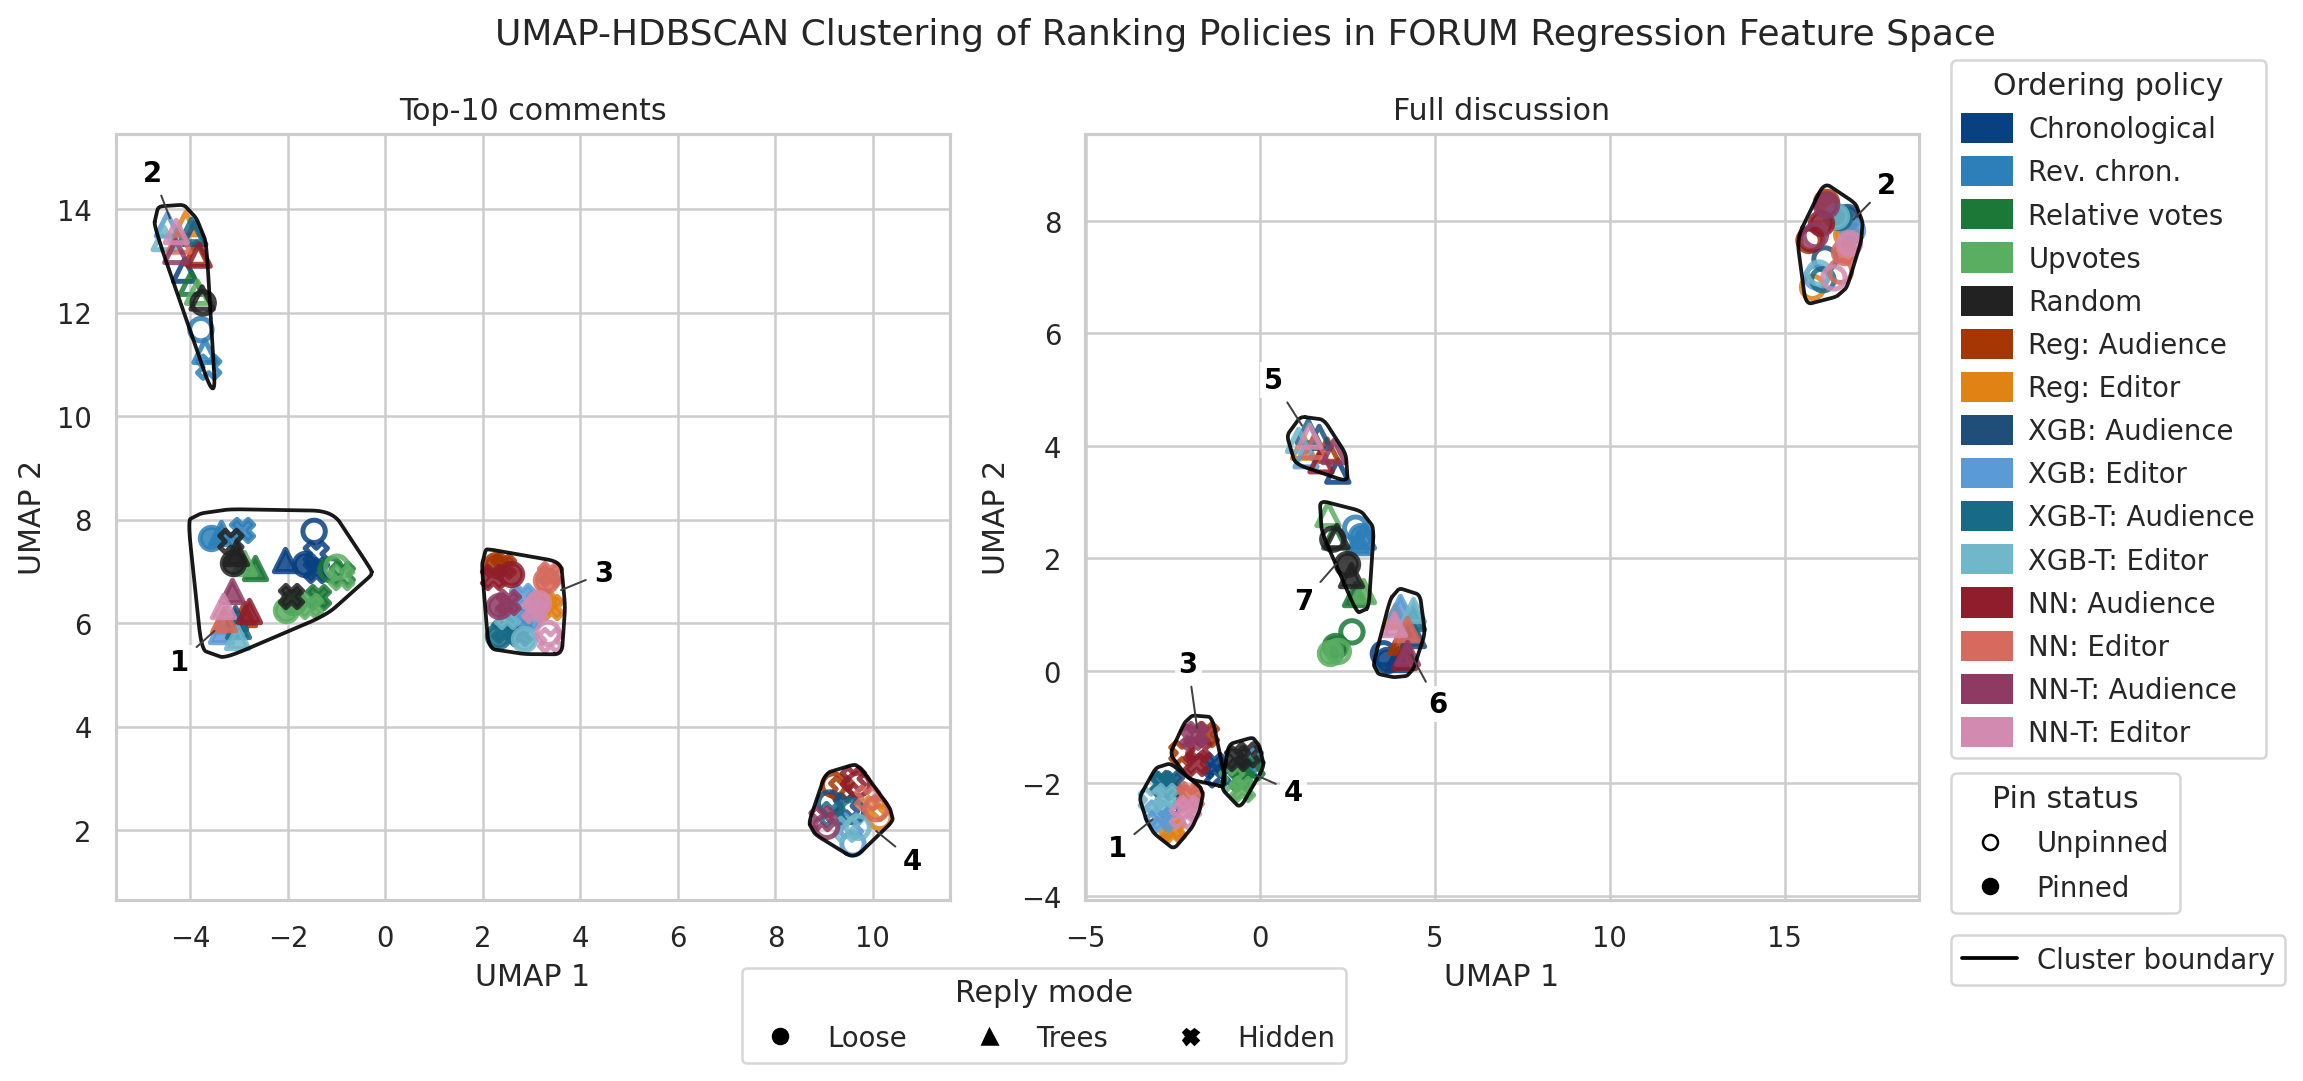
\includegraphics[width=\linewidth]{figures/policy_umap_hdbscan.png}
\caption{UMAP--HDBSCAN clustering of policies in FORUM regression-feature space, separately at top 10 and full depth. Clusters are fitted in ten-dimensional UMAP space and displayed in a separate two-dimensional UMAP embedding.}
\label{fig:policy-clusters}
\end{figure*}

\subsubsection{Article versus relative-vote agenda gains}
The two-target comparison shows that article-directed movement is not simply movement toward any salient agenda (Figures~\ref{fig:target-gain-effects} and \ref{fig:target-gain-scatter}). For every predictive model, the marginal effect on article gain exceeds its effect on relative-vote gain, with all ten paired difference intervals above zero. The regression-editor difference is $+0.0076$ (95\% CI 0.0060--0.0092); corresponding differences are $+0.0064$ for XGBoost editor ordering (0.0047--0.0079) and $+0.0075$ for neural editor ordering (0.0058--0.0092). The text-enabled editor differences remain positive, $+0.0045$ for XGBoost (0.0030--0.0060) and $+0.0056$ for the neural model (0.0040--0.0073). The article-optimising oracle gains $0.0860$ towards the article and $-0.0241$ towards the vote-derived agenda, giving an article-minus-vote benchmark of $0.1100$ in the combined figure. This ordering was optimised for article alignment, not for the gain difference.

This pattern has clear limits. The relative-vote and upvote ordering contrasts favour the vote-derived target (as one would expect), with article-minus-vote differences of $-0.0018$ ($-0.0031$ to $-0.0005$) and $-0.0020$ ($-0.0034$ to $-0.0008$). Chronological ordering also has a negative difference, while reverse chronology is inconclusive. Hiding replies strongly favours the article target ($+0.0474$, 0.0429--0.0518), but retaining discussion trees favours the vote-derived target ($-0.0028$, $-0.0036$ to $-0.0021$). Pinning's two-target difference spans zero. Thus the evidence supports stronger article-directed effects for predictive model and hidden-reply presentation, rather than for every interface decision.

For the complete default policy, mean article gain against random/loose/unpinned presentation is $0.0118$ (95\% CI $0.0097$--$0.0140$), compared with $0.0023$ ($0.0015$--$0.0031$) towards the relative-vote agenda. The paired article-minus-vote gain is $0.0095$ ($0.0074$--$0.0117$), across 2,530 discussions with valid gains for both targets. Thus the default moves towards both reference agendas, with a larger gain towards the article. These bundle-level gains correspond to a point in Figure~\ref{fig:target-gain-scatter}, rather than a marginal effect in Figure~\ref{fig:target-gain-effects}.

\begin{figure}[t]
\centering
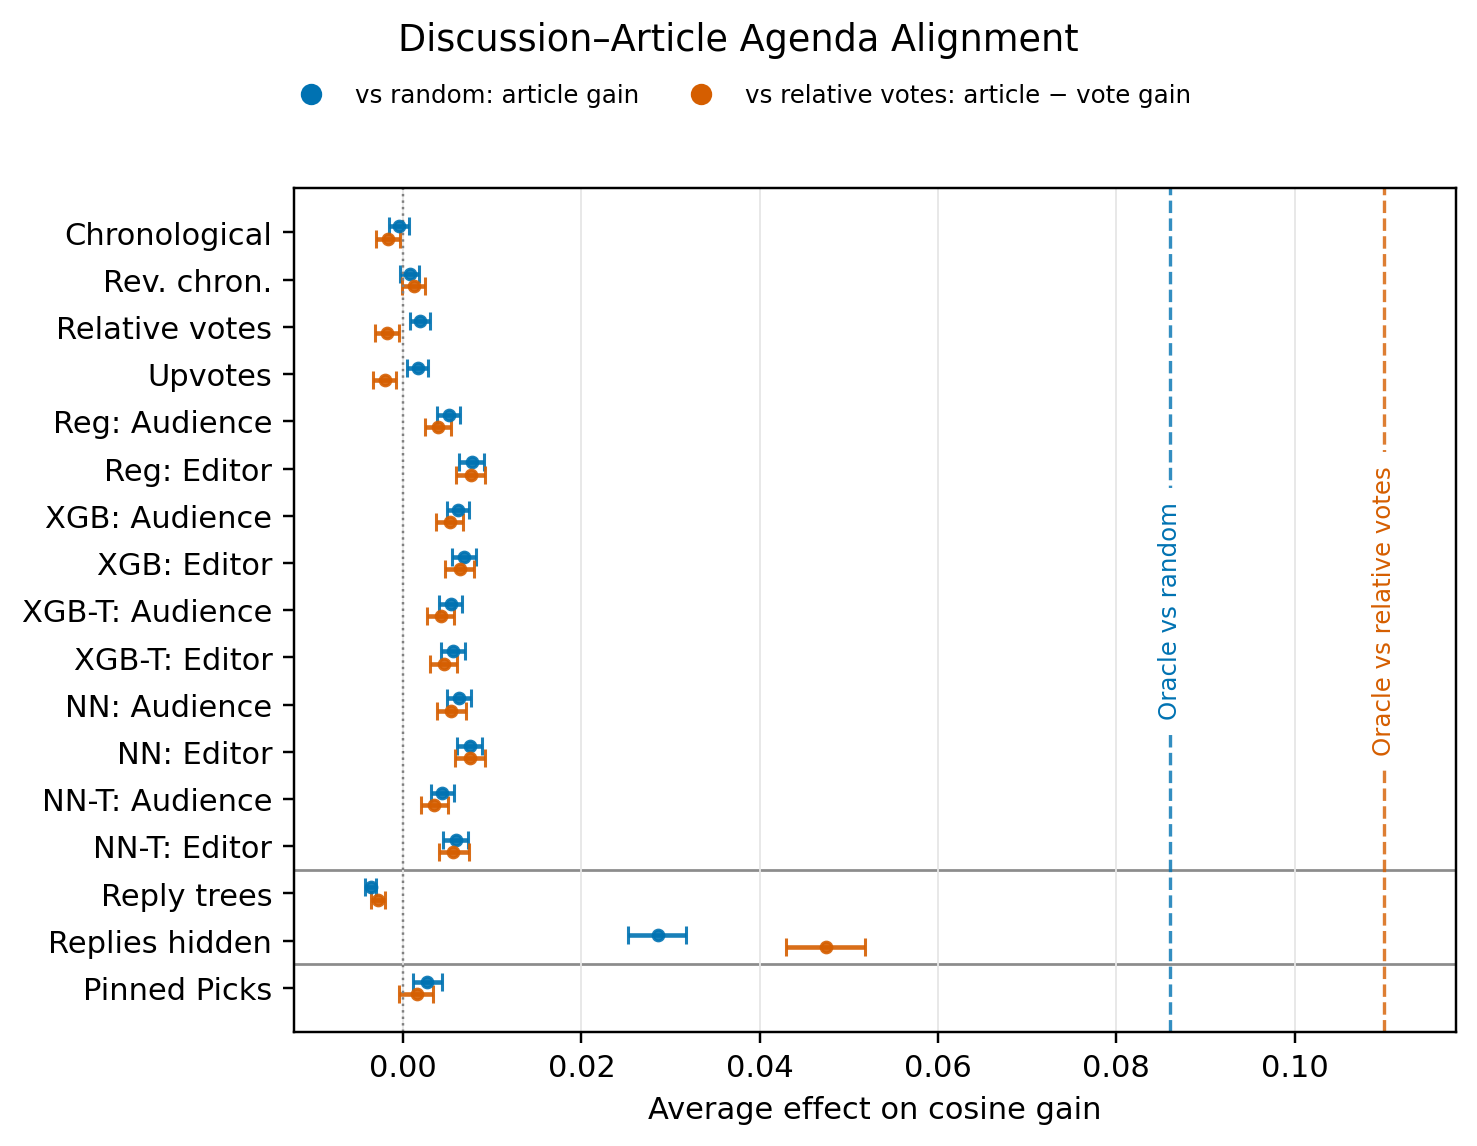
\includegraphics[width=\linewidth]{figures/topic_combined_article_cosine_gain_effects.png}
\caption{Average policy effects on article gain versus random and article-minus-relative-vote gain. Both series use paired ordering and interface contrasts; points and intervals are 95\% discussion-bootstrap intervals.}
\label{fig:article-cosine-gain}
\label{fig:target-gain-effects}
\end{figure}

\begin{figure}[t]
\centering
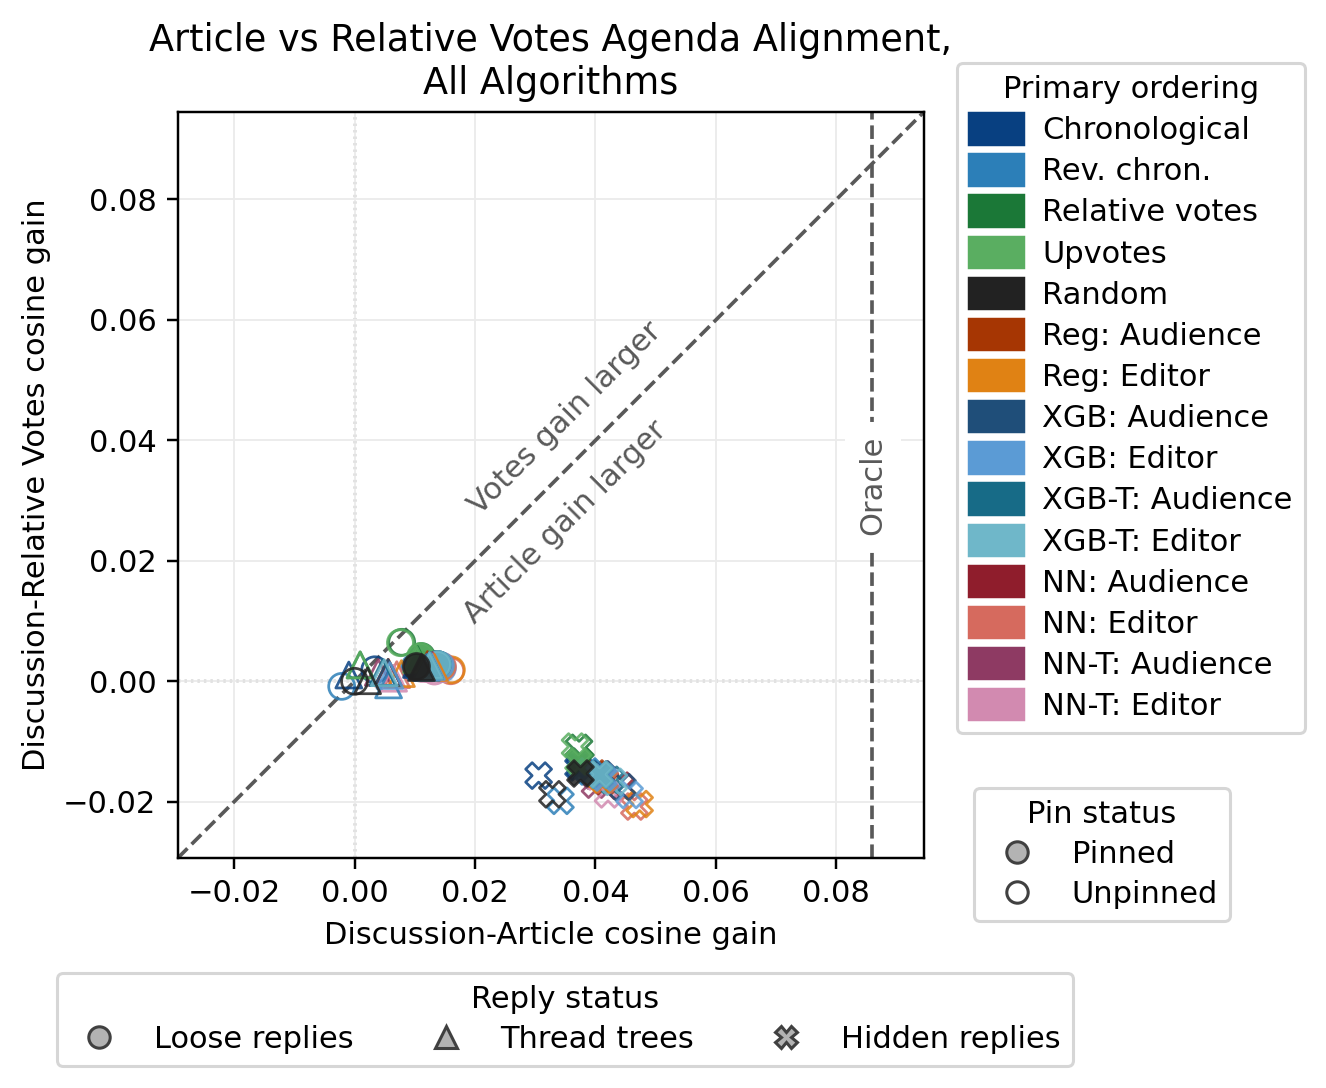
\includegraphics[width=\linewidth]{figures/article_relative_votes_raw_gain_scatter.png}
\caption{Mean cosine gains toward the article and relative-vote topic agenda for all 90 ranking algorithms.}
\label{fig:target-gain-scatter}
\end{figure}

\section{Discussion}
Ranking policy is an editorial-governance decision about the representation of an existing comment pool. Journalists exert curatorial gatekeeping through the comments they pin, while ordering and reply handling shape the surrounding discussion. Our results show how these choices alter both the attributes brought forward (RQ1) and the topics receiving prominence (RQ2).

For RQ1, predictive models promote AQuA, article similarity, and lexical diversity; interface choices can offset these gains. These outcomes overlap with ranker inputs, so gains do not independently validate quality. Because only 29.7\% of candidates are roots, reply handling is consequential: trees preserve context but constrain early prominence, whereas hiding replies increases article alignment while reducing full-discussion AQuA. These trade-offs, and differences between top-10 and full-discussion results, show why ranking audits must specify both interface and evaluation depth.

Pinning gives editors targeted control over early prominence. Editors' Picks account for only 0.87\% of comments, with an average of four per discussion, yet occupy the first positions when pinned. Their feature effects are small in comparison to full discussion ordering or reply handling, yet one must bear in mind that this is an intervention over a very small number of comments. Pinning effects can change direction over the full discussion: the AQuA FORUM contrast is positive at top 10 ($0.0294$, 95\% CI $0.0235$--$0.0355$) but negative at full depth ($-0.0197$, $-0.0216$ to $-0.0177$). Future research could examine if larger curated selections change this relationship.

Greater article alignment can come with lower deliberative quality: hiding replies increases article alignment while reducing full-discussion AQuA. Further work should examine how these trade-offs affect conversation interpretability and reader experience, including the value of seeing a contribution alongside the comment it answers.

For RQ2, the topic analysis shows that predictive models yield larger article-directed than relative-vote-directed gains in the paired ordering contrasts. Hiding replies strengthens article alignment further and shifts it away from the vote-derived agenda. A newsroom can therefore obtain a more article-focused presentation at the expense of breadth and the prominence of issues introduced or endorsed by commenters. Pinning does not show the same consistent conclusive preference between the two targets.

Neither target provides a neutral account of public opinion. The article distribution reflects the issues covered in the story, while the relative-vote distribution reflects participating voters under existing exposure conditions. Topical agreement also does not imply agreement in viewpoint. A newsroom seeking rapid orientation may choose differently from one seeking to preserve extended disagreement and exchange. We advise against optimising solely for one FORUM score or agenda. The sizeable effects for predictive models show their capacity to reshape a discussion, but whether a change improves participation or readers' understanding requires behavioural evidence. These questions also apply to news discussion on social media, where ranking may play an even wider role in allocating visibility.

Changes in topic prominence and visible comment attributes correspond to potential first- and second-level agenda-setting mechanisms, respectively; because we measure presentation rather than audience response, their behavioural effects remain to be established.

Our versatile FORUM score can be applied in future research, including different news platforms and experimental studies on ranking algorithms' impact on user behaviour. It can also be used to study ranking in other contexts where a finite set of items, each with measurable features, is ordered by a potentially unknown algorithm. Examples include news feeds, social media comments, job postings, and product listings. In each case, the choice of features and the treatment of omitted items must reflect the setting being studied.

\section{Limitations and Ethical Considerations}
\label{sec:ethics}

We measure presentation rather than behavioural response on one German-language forum, limited to discussions containing Editors' Picks. Generalisation and causal effects require studies on other platforms and experimental or policy-change designs. Our snapshot also omits changes over time in votes, pinning, and deletions.

Topic assignments depend on the embedding model, mixed fitting sample, and clustering choices. Only 26.64\% of comments receive a valid assignment, so the topic results describe the assigned portion of discussion. The relatively high proportion of unassigned comments is unsurprising given the large number of short, non-substantive comments in the corpus. Yet, these comments may contain implicit endorsement of specific viewpoints or agenda issues (e.g. "We should be talking more about this!"). The topic model is also not a measure of political diversity or agreement.

The study received institutional ethics review approval (ID 13838441). The project follows the Association of Internet Researchers' ethics framework \citep{AoIR2019} and, whilst it is not feasible or methodologically prudent to seek informed consent at scale, considers contextual privacy and potential harm throughout the research process. Data collection followed the site's robots.txt directives and terms \citep{DerStandard2024, DerStandardRobots2026}. The collector retrieved public records without posting comments, voting, or otherwise participating in discussions. Author identifiers were replaced by hashed pseudonyms during collection. This enables longitudinal linkage but does not anonymise the data: verbatim text, timestamps, and histories may remain identifying or searchable. We share code, documentation, and aggregate results while withholding the full comment-level dataset to reduce risks to commenters' privacy.

Ranking audits can support more transparent moderation, but the same methods could be used to suppress viewpoints or engineer apparent consensus. Their appropriate use requires explicit objectives and disclosure of measurement limits. Newsrooms should make the purpose of ranking legible to readers and consider whose contributions lose prominence. Article alignment and automated quality scores should not be treated as grounds for excluding legitimate criticism; preserving routes to wider discussion can help readers assess comments for themselves.

\section{Conclusion}
This paper examines the representational consequences of comment ranking on a large news website. FORUM measures how policies promote or suppress comment attributes, while topic modelling assesses changes in the topical focus of the presented discussion. For RQ1, predictive models bring forward deliberative quality, article similarity, and lexical diversity, but reply handling can offset these gains, and early prominence differs from full-discussion presentation. For RQ2, predictive models show stronger article-directed than vote-directed marginal gains, while hiding replies further intensifies article alignment.

Journalists retain direct editorial influence through pinned Editors' Picks, but ordering and reply handling also shape which contributions receive prominence. No single policy is best across the measured attributes and agendas. Newsrooms must choose in light of their purposes for discussion, while researchers and readers need to account for display rules when interpreting visible responses to news.

News comments allow readers to contribute knowledge, experience, and criticism to journalism. Making the consequences of ranking explicit can help newsrooms support that participation while attending to contributions that their chosen presentation leaves less visible.

\section*{Acknowledgments}
OpenAI Codex was used in co-writing analysis code and reorganising author-written manuscript text.
